\documentclass[a6paper,10pt,twoside]{article}
%\usepackage[T1]{fontenc}
\usepackage[british]{babel}
\usepackage[utf8]{inputenc}
\usepackage{float, graphicx,amsmath,amsfonts,cite,enumerate,ulem}
\usepackage[final]{pdfpages}
\usepackage{wrapfig}
\usepackage[margin=0.3in]{geometry}
\usepackage{sidspaltHack}
\usepackage{digital}

\setlength{\evensidemargin}{-0.47in}
\setlength{\oddsidemargin}{-0.37in}
\setlength{\textwidth}{215pt}

\pagestyle{empty}

\begin{document}
\nysida{12}{1}
\noindent
\chaptertitlenobr{M$\mu$}{Nidvisor}
\small
\begin{center}
\songtitle{$\mu1$}{Jag har aldrig vart på snusen}
\mel{Åh, hur saligt att få vandra}
\end{center}
\begin{lyrics}
Jag har aldrig vart på snusen,\\
aldrig rökat en cigarr, haleluja!\\
Mina dygder äro tusen,\\
inga syndiga laster jag har.\\
Jag har aldrig sett nå't naket,\\
inte ens ett litet nyfött barn.\\
Mina blickar går mot taket,\\
därmed undgår jag frestarens garn.
\vspace{5pt}\\
Haleluja - haleluja...
\vspace{5pt}\\
Bacchus spelar på gitarren,\\
satan spelar på sitt handklaver.\\
Alla djävlar dansar tango,\\
säg vad kan en väl önska sig mer?\\
Jo, att alla bäckar vore brännvin,\\
Riddarfjärden full av bayerskt öl.\\
Konjak i varenda rännsten\\
och punsch i varenda vattenpöl.
\vspace{5pt}\\
Och mellanöl - och mellanöl... 
\end{lyrics}

\nysida{12}{2}
\noindent
\begin{center}
\songtitle{$\mu2$}{Handelsvisa}
\mel{Åh, hur saligt att få vandra}
\end{center}
\begin{lyrics}
Jag vill aldrig gå på Handels,\\
aldrig tenta företagsekonomi.\\
Deras IQ den e' Mandels\\
och förståndet, det har ju gjort sorti.\\
Dom har jätteusla snören\\
till sitt jätteusla draperi.\\
Dom kan bara räkna ören,\\
hela skolan e' ett enda aperi!
\vspace{5pt}\\
Handels är skit - Jag vill ej dit...
\vspace{5pt}\\
Mammons pojkar är dom alla,\\
pappas flickor är dom likaså.\\
Går och tror att dom är balla,\\
fastän dom inget alls ju förstå.\\
Hela Handels borde rivas,\\
detta anser hela vårat lag.\\
Då skulle Osquarulda trivas.\\
uppå denna Handels ljuva domedag!
\vspace{5pt}\\
Åh, vilket drag - på denna dag... 
\end{lyrics}
\auth{Team kangaroo Gerhards-gasque 1977}

\nysida{12}{3}
\noindent
\begin{center}
\songtitle{$\mu3$}{Fysikhatarvisan}
\mel{Åh, hur saligt att få vandra}
\end{center}
\begin{lyrics}
Jag vill inte gå på fysik,\\
aldrig tenta termometerdynamik.\\
Jag vill inte höra syntmusik,\\
inte festa som en tråkig mattegeek.\\
Vi ser ut som Televerket\\
i vår jättefula overall.\\
Vi kan bara räkna kvarkar,\\
nu hyllar vi Data med en skål!
\vspace{5pt}\\
Fysik är torrt - jag vill ju bort!
\vspace{5pt}\\
Einsteins vänner är vi alla.\\
Handelsmänn'skor kan vi aldrig få.\\
Går och tror att vi är balla,\\
det får bli på egen hand om det ska gå.\\
Nu ska hela Sing-Sing rivas,\\
Arkitekt är med på Datas lag.\\
Televerket ska fördrivas\\
uppå Konsulatets ljuva domedag.
\vspace{5pt}\\
Å nubbedrag - på denna dag... 
\end{lyrics}
\auth{DKM hösten 2000}

\nysida{12}{$\pi$}
\noindent
\begin{center}
\songtitle{$\mu\pi$}{Matematikhatarvisan}
\mel{Åh, hur saligt att få vandra}
\end{center}
\begin{lyrics}
Varför valde jag ens matte?\\
Kunde jag inte bara valt mediateknik\\
Härligt softa med en latte\\
Behövde jag vara så unik\\
Fattat nada sen vår första lektion\\
Men ändå ska vi kunna varenda skumma ekvation\\
Derivera någon skum funktion\\
Detta kommer ge mig depression
\vspace{5pt}\\
$\|$: Matten är skum - känner mig dum!\\
Kan jag förstå - haha nejdå!\\
Endast aptit - för akvavit!\\
Jag tar en bit! :$\|$
\vspace{5pt}\\
Vad har kor för aerodynamik\\
Vad är däckens optimala mönsterdjup\\
Ha så kul med detta på fysik\\
Svaret blir att ni ska ta en sup \textit{(alla fysikare dricker)}\\
Lär sig snillen ragga tjejer/killar\\
Nej vi lär oss inget annat praktiskt heller\\
Bara många skumma grejer/Bara sånt vi inte gillar\\
Ingen förstår vad vi säger/IQ:n densamma som sillar
\vspace{5pt}\\
$\|$: Pytagoras sats - Eulers sats!\\
Rolles sats - cosinussats!\\
Spelar roll? - Har ingen koll!\\
Allting blir noll! :$\|$
\end{lyrics}
\auth{Lukas Granqvist, Axel Abrahamsson\\ \sout{Jongasquen} Jonpicknicken 2020}

\nysida{12}{4}
\noindent
\begin{center}
\songtitle{$\mu4$}{Datas visa}
\mel{Åh, hur saligt att få vandra}
\end{center}
\begin{lyrics}
\vspace{-5pt}
Alla de som går på Data\\
sitter mest och kodar Perl-script varje natt.\\
Med dem kan en inte prata\\
om en inte loggat in på någon chatt.\\
Deras hy är grå som aska,\\
när solen skiner sysslar de med webdesign.\\
Och när vi andra börjat gasqua\\
sitter de och spelar Ultima Online.
\vspace{5pt}\\
$\|$: Datan är grå - visst är det så!\\
Datan är trist - javisst, javisst!\\
Datan är skit - en drar en nit\\
om en går dit! :$\|$
\vspace{5pt}\\
De har något tomt i blicken,\\
en hel skvadron av tomtar på sitt loft!\\
Ingen av dem har nån partner,\\
men de drömmer varje natt om Lara Croft.\\
Data borde formateras,\\
systematiskt, partition för partition.\\
Nördarna dekompileras\\
och uppgraderas till en användbar version.
\vspace{5pt}\\
Datan är grå...
\end{lyrics}
\vspace{-5pt}
\begin{figure}[!h]
\begin{minipage}{0.5\linewidth}
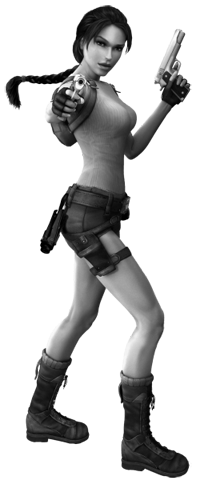
\includegraphics[width=0.37\textwidth]{lara_croft.png}
\end{minipage}
\begin{minipage}{0.48\linewidth}
\auth{Mattis Castegren (D)\\ Ettans fest 2001}
\end{minipage}
\end{figure}


\nysida{12}{5}
\noindent
\begin{center}
\songtitle{$\mu5$}{Hyllningsvisa}
\mel{Sit on my face}
\end{center}
\begin{lyrics}
Teknik fysik är mössbeklädda töntar,\\
mammas pojkar och en samling pappas flickor.\\
Liknar mest en televerksbil, som gått för många mil,\\
en teknisk fossil.
\vspace{5pt}\\
Teknisk Fysik är lättare än att fjärta,\\
döda älgar värmer nu mitt kalla hjärta.\\
Ta hit dynamit, sprängteknik vårt gebit!\\
$\|$: Dessa tofsprydda avskum som ger oss kolik!:$\|$\textit{(3 ggr)}
\begin{center}
\textit{Sjunges tre gånger medan tofsen snurras i cirklar. Bärs ej mössa, så låtsas en och snurrar i luften.\\ Därefter:}
\end{center}
Dessa tekniska lik!!! Barampam!
\begin{center}
\textit{På Barampam lyftes mössan, alternativt luften ovanför hjässan, i hälsning.}
\end{center}
\end{lyrics}
\auth{V - LTH}

\nysida{12}{6}
\noindent
\begin{center}
\songtitle{$\mu6$}{En ska gå Teknis}
\mel{Husvagn}
\end{center}
\begin{lyrics}
Jag har prövat nästan allt som finns att välja på:\\
Sjukgymnastik, historia är inge' kul att gå.\\
Jag har studerat på de allra konstigaste sätt\\
och äntligen jag funnit hur en ska studera rätt.
\vspace{5pt}\\
En ska gå Teknis, och läsa matte och fysik.\\
En ska gå Teknis, då har jag hört att en blir rik.\\
En ska gå Teknis, och flytta in på KTH.\\
För att på Teknis, där vill alla gå!
\vspace{5pt}\\
I många år så var vi faktiskt bland de allra bästa,\\
men nu så är vi sämst, så vi kan lika gärna festa.\\
Föhseriet säger n$\emptyset$llan är schlemmig och w$\ddot{u}$drogh,\\
så'n tur att fadderiet plocka' upp oss där vi låg.
\vspace{5pt}\\
En ska ha faddrar, som står och väntar utanför.\\
En ska ha faddrar, som alltid visar hur en gör.\\
En ska ha faddrar, som en kan krama på ibland.\\
Ja våra faddrar, ror ju allt i land!
\vspace{5pt}\\
5 minuter övningsgasque och 5 minuter draqueflyg,\\
5 minuter Kårens dag och Föhseriets otyg,\\
5 minuter intromatte och 5 minuter vals.\\
Bäsk å punsch å andra drycker fyller våran hals.
\vspace{5pt}\\
En ska gå Teknis, och läsa matte och fysik.\\
En ska gå Teknis, då har jag hört att en blir rik.\\
En ska gå Teknis, och flytta in på KTH.\\
För att på Teknis, där vill alla gå!
\end{lyrics}
\auth{Tjejn$\emptyset$llan, FanFar}

\nysida{12}{7}
\noindent
\begin{center}
\songtitle{$\mu7$}{Teknologvisa}
\mel{Lumberjack song}
\textit{Försångare / \textbf{Alla}}
\end{center}
\begin{lyrics}
Jag är teknolog och helt OK,\\
jag jobbar hårt och jag roar mig.\\
\textbf{Hen är teknolog och helt OK,\\
hen jobbar hårt och hen roar sig.}
\vspace{5pt}\\
Teknik är ball,\\
jag kan Pascal.\\
Till Lophtet vill jag gå,\\
där träffas alla vänner\\
som är från LTH.
\vspace{5pt}\\
\textbf{Teknik är ball,\\
hen kan Pascal.\\
Till Lophtet vill hen gå,\\
där träffas alla vänner\\
som är från LTH.
\vspace{5pt}\\
För hen är teknolog och helt OK,\\
hen jobbar hårt och hen roar sig.}
\vspace{5pt}\\
Min mattebok, den gör mig klok.\\
Jag läser kärnfysik.\\
Jag går på föreläsning\\
och älskar juridik.
\vspace{5pt}\\
\textbf{Hens mattebok, den gör henom klok.\\
Hen läser kärnfysik.\\
Hen går på föreläsning\\
och älskar juridik. \textit{(förvånat)}
\vspace{5pt}\\
Men hen är teknolog och helt OK,\\
hen jobbar hårt och hen roar sig.}
\vspace{5pt}\\

\newpage
\noindent
Som ekonom jag blir fantom.\\
Konkurser gör mig säll.\\
Till flickor blankt jag nekar.\\
Jag älskar en tabell.
\vspace{5pt}\\
\textbf{Som ekonom hen blir fantom \textit{(förvånat)}\\
konkurser...\\
Nää, BUU!!!
\vspace{5pt}\\
Men hen är teknolog och helt OK,\\
hen jobbar hårt och hen roar sig.}
\end{lyrics}

\vspace{20pt}
\begin{figure}[!h]
\hspace{30pt}
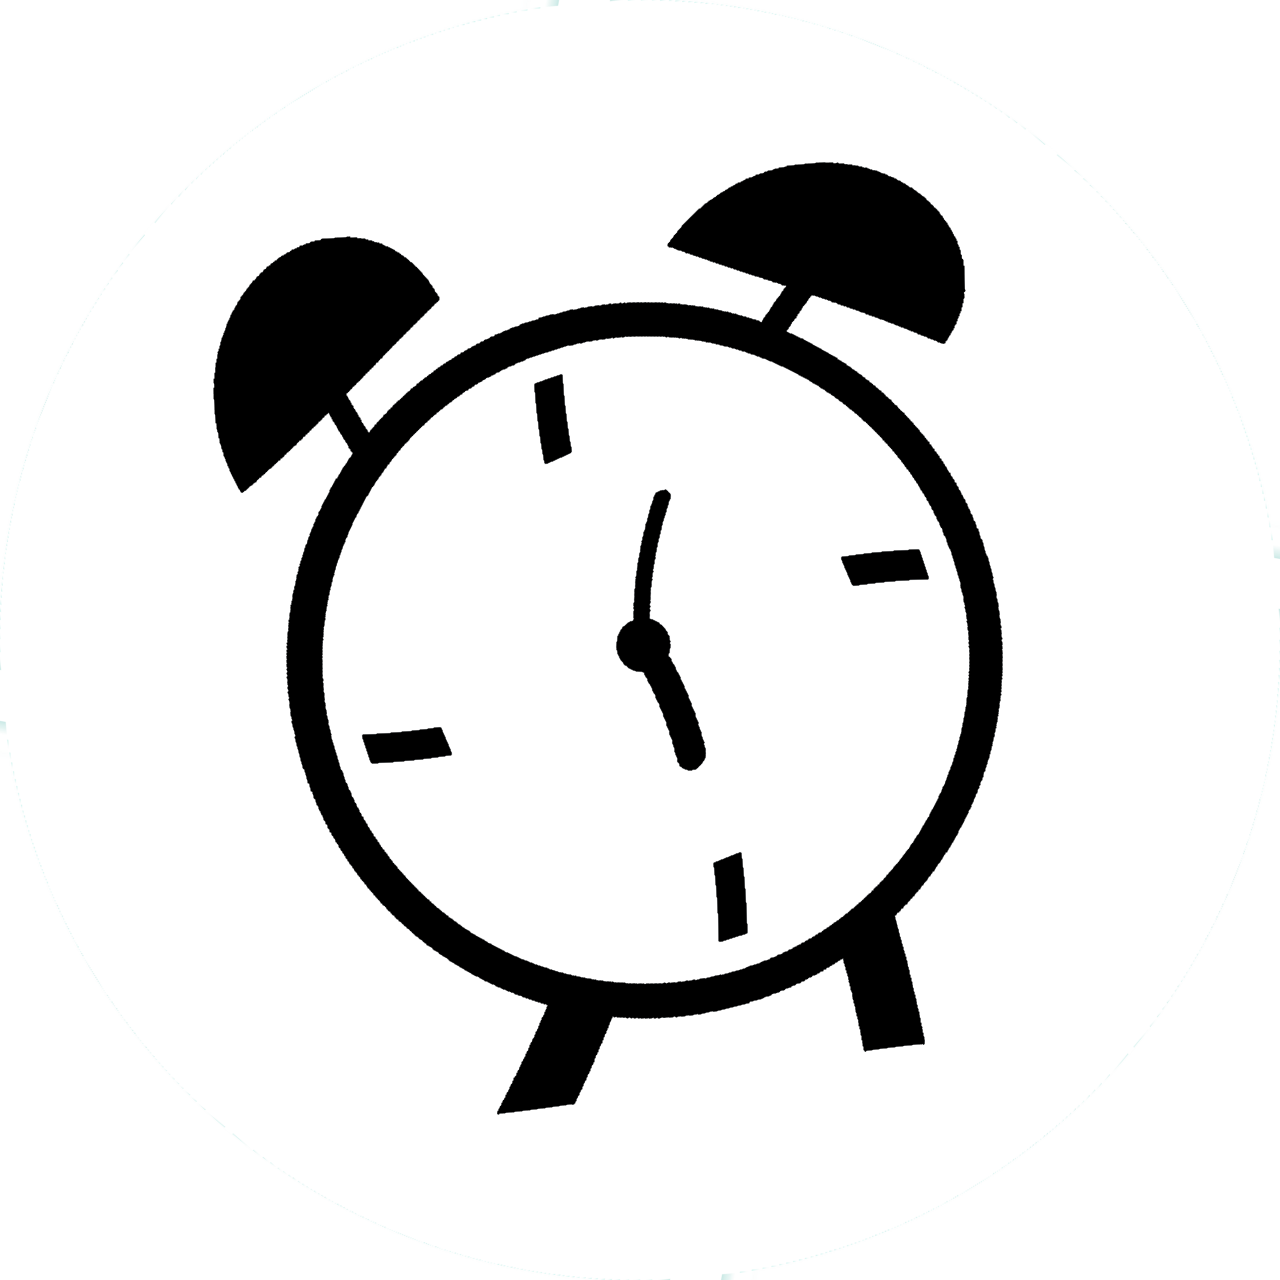
\includegraphics[width=0.70\textwidth]{klocka.png}
\end{figure}

\nysida{12}{8}
\noindent
\begin{center}
\songtitle{$\mu8$}{Teknologen och ekonomen}
\mel{Katyuscha}
\end{center}
\begin{lyrics}
Teknologen vaknar upp en morgon, \\
klockan visar tio över sex. \\
Ekonomen ligger kvar i sängen, \\
snarkar så hen borde ha komplex.
\vspace{5pt} \\
Na na na na...
\vspace{5pt} \\
Teknologens cykel har punktering, \\
lagas lätt man gaffar lite på’n! \\
Ekonomen ligger kvar i sängen. \\
Cykeln hens, den är i Fyrisån.
\vspace{5pt} \\
Na na na na... 
\vspace{5pt} \\
Teknologen labbar åtta timmar. \\
Teknologen är rätt nöjd ändå. \\
Ekonomen ligger kvar i sängen, \\
hade faktiskt EN lektion igår!
\vspace{5pt} \\
Na na na na...
\vspace{5pt} \\
Teknologen ska på fest på kvällen, \\
putsar lite på sin overall. \\
Ekonomen ligger kvar i sängen, \\
vaknar inte ens av Flogstavrål.
\vspace{5pt} \\
Na na na na... 
\vspace{5pt} \\
Teknologen plockar ut examen. \\
Nu är hen en riktig sexikon. \\
Ekonomen ligger kvar i sängen... \\
... somnar när hen ser sitt lexikon! 
\end{lyrics}
\auth{Uppsala teknolog- och naturvetarkårs sångbok}



%\begin{center}
%\Large $\mu$5. Orangea overaller\\
%\mel{Bananer i pyjamas}
%\end{center}
%Orangea overaller, dom har vi tagit på\\
%Orangea overaller, dom stojar och står på\\
%Orangea overaller, dom skojar och har fest
%Orangea overaller, dom vrålar F ÄR BÄST!
%\begin{flushright}
%\textit{Bl. a. Björn Ardö F98 (Lund)}
%\end{flushright}

\end{document}